\documentclass[twoside]{article}
\usepackage[a4paper]{geometry}
\geometry{verbose,tmargin=2.5cm,bmargin=2cm,lmargin=2cm,rmargin=2cm}
\usepackage{fancyhdr}
\pagestyle{fancy}

% nastavení pisma a~češtiny
\usepackage{lmodern}
\usepackage[T1]{fontenc}
\usepackage[utf8]{inputenc}
\usepackage[czech]{babel}

% odkazy
\usepackage{url}

\usepackage{float}
% vícesloupcové tabulky
\usepackage{multirow}
\usepackage{listings}
\usepackage{xcolor}
\usepackage{amssymb}
\usepackage{gensymb}
\usepackage{bbold}
\usepackage{amsmath}
\usepackage{siunitx}
\usepackage{mathtools}
\usepackage{commath}

% vnořené popisky obrázků
\usepackage{subcaption}

% automatická konverze EPS 
\usepackage{graphicx} 
\usepackage{epstopdf}
\epstopdfsetup{update}

\graphicspath{{./images}}

% odkazy a~záložky
\usepackage[unicode=true, bookmarks=true,bookmarksnumbered=true,
bookmarksopen=false, breaklinks=false,pdfborder={0 0 0},
pdfpagemode=UseNone,backref=false,colorlinks=true] {hyperref}


% Poznámky při překladu
\usepackage{xkeyval}	% Inline todonotes
\usepackage[textsize = footnotesize]{todonotes}
\presetkeys{todonotes}{inline}{}

%https://tex.stackexchange.com/questions/2783/bold-calligraphic-typeface
\DeclareMathAlphabet\mathbfcal{OMS}{cmsy}{b}{n}

% enumerate zacina s pismenem
\renewcommand{\theenumi}{\alph{enumi}}

% smaz aktualni page layout
\fancyhf{}
% zahlavi
\usepackage{titling}
\fancyhf[HC]{\thetitle}
\fancyhf[HLE,HRO]{\theauthor}
\fancyhf[HRE,HLO]{\today}
 %zapati
\fancyhf[FLE,FRO]{\thepage}

% údaje o autorovi
\title{OTE Domácí úkol 2 - Zesilovače}
\author{Vojtěch Michal}
\date{\today}

%customize code listing
\definecolor{codegreen}{rgb}{0,0.6,0}
\definecolor{codegray}{rgb}{0.5,0.5,0.5}
\definecolor{codepurple}{rgb}{0.58,0,0.82}
\definecolor{backcolour}{rgb}{0.95,0.95,0.92}

\lstdefinestyle{mystyle}{
    backgroundcolor=\color{backcolour},   
    commentstyle=\color{codegreen},
    keywordstyle=\color{magenta},
    numberstyle=\tiny\color{codegray},
    stringstyle=\color{codepurple},
    basicstyle=\ttfamily\footnotesize,
    breakatwhitespace=false,         
    breaklines=true,                 
    captionpos=b,                    
    keepspaces=true,                 
    numbers=left,                    
    numbersep=5pt,                  
    showspaces=false,                
    showstringspaces=false,
    showtabs=false,                  
    tabsize=2
}

\lstset{style=mystyle}

\begin{document}

\maketitle

V simulacích pro tuto úlohu bylo použito nastavení parametrů operačního zesilovače uvedené v tabulce \ref{tab:oz_param}.
Symbolem $u_2$ označuji napětí na výstupu operačního zesilovače proti zemi.

\begin{table}[h!]
    \centering
    \begin{tabular}{c|c|c|c|c}
        parametr & symbol & hodnota & jednotka & poznámka\\
        \hline
        Vstupní napěťový offset & $U_0$ & 1 & \si{\milli\volt} & \\
        Vstupní klidový proud & $I_\text{B}$ & 50 & \si{\nano\ampere} & $(I_\text{BP} + I_\text{BN})/2$ \\
        Vstupní zbytkový proud & $I_0$ & 20 & \si{\nano\ampere} & $I_\text{BP} - I_\text{BN}$ \\
        Zesílení v otevřené smyčce & $A_\text{D}$ & 200 & \si{\kilo\volt\per\volt} & \\
        Tranzitní kmitočet& $f_T$ & 1 & \si{\mega\hertz} &
    \end{tabular}
    \caption{Parametry operačního zesilovače použité pro simulaci}
    \label{tab:oz_param}
\end{table}

\section{Napěťový sledovač}

Multimetrem byly změřeny hodnoty statických parametrů operačního zesilovače.
Zapojením sledovače napětí a připojením neinvertujícího vstupu na zem podle schématu \ref{fig:sledovac_voltage_offset}
bylo změřeno zbytkové napětí
\begin{equation}
    U_0 = 999.995 \mu \text{V} \approx 1 \si{\milli\volt}.
\end{equation}

\begin{figure}[h!]
    \centering
    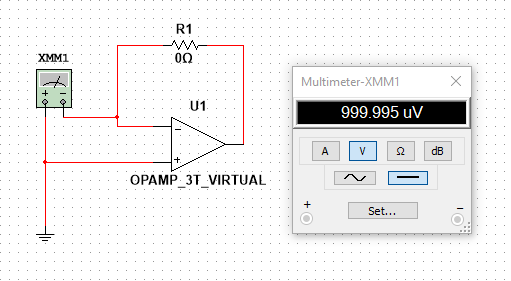
\includegraphics[width=\linewidth]{sledovac_voltage_offset.png}
    \caption{Zapojení pro změření zbytkového napětí OZ}
    \label{fig:sledovac_voltage_offset}
\end{figure}


\begin{figure}
    \centering
    \begin{subfigure}{0.45 \textwidth}
        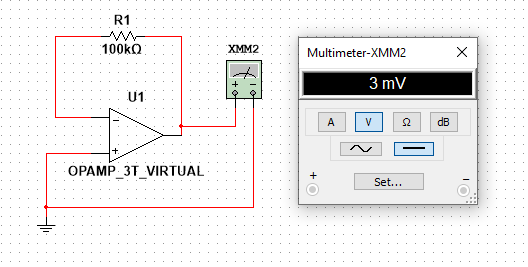
\includegraphics[width=\linewidth]{sledovac_IBN.png}
        \caption{Zapojení pro měření $I\text{BN}$}
        \label{fig:sledovac_IBN}        
    \end{subfigure}
    \begin{subfigure}{0.45\textwidth}
        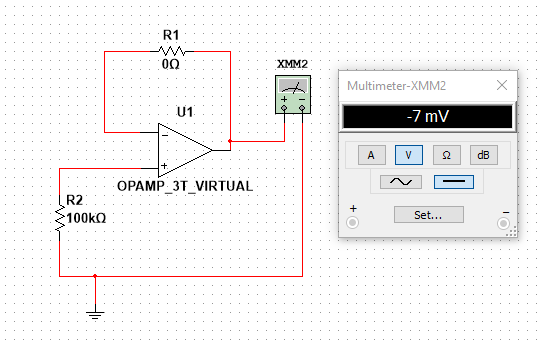
\includegraphics[width=\linewidth]{sledovac_IBP.png}
        \caption{Zapojení pro měření $I\text{BP}$}
        \label{fig:sledovac_IBP}
    \end{subfigure} \hfil
    \caption{Měření vstupních proudů svorek OZ}
\end{figure}

Zapojením rezistoru $R_1 = 100 \si{\kilo\ohm}$ do záporné zpětné vazby dle schématu \ref{fig:sledovac_IBN} byl změřen
vstupní proud invertující svorky
\begin{equation}
    I_\text{BN} = \frac{u_2 - U_0}{R_1} = \frac{3 \si{\milli\volt} - (-1 \si{\milli\volt})}{100 \si{\kilo\ohm}}
    = 4 \cdot 10^{-5-3} \si{\ampere} = 40 \si{\nano\ampere}.
\end{equation}

Zapojením rezistoru $R_2 = 100 \si{\kilo\ohm}$ mezi neinvertující vstup a zem dle schématu \ref{fig:sledovac_IBP}
byl změřen vstupní proud neinvertující svorky
\begin{equation}
    I_\text{BP} = -\frac{u_2 + U_0}{R_2} = -\frac{-7 \si{\milli\volt} + 1 \si{\milli\volt}}{100 \si{\kilo\ohm}}
    = 6 \cdot 10^{-5-3} \si{\ampere} = 60 \si{\nano\ampere}.
\end{equation}

Odtud lze vypočíst velikosti vstupního zbytkového proudu
\begin{equation}
    I_0 = I_\text{BP} - I_\text{BN} = 20 \si{\nano\ampere}
\end{equation}
a vstupního klidového proudu
\begin{equation}
    I_\text{B} = \frac{I_\text{BP} + I_\text{BN}}{2} = 50 \si{\nano\ampere},
\end{equation}
které přesně odpovídají parametrům nastaveným dle tabulky \ref{tab:oz_param}.

\section{Neinvertující zesilovač}

Zadaných zesílení 2 a 11 lze s neinvertujícím zesilovačem dosáhnout
fixováním $R_2 = 10 \si{\kilo\ohm}$ a použitím
$R_1 \in \left\{10, 100\right\} \si{\kilo\ohm}$ dle schématu \ref{fig:neinv_zesilovac}.

\begin{figure}[h!]
    \centering
    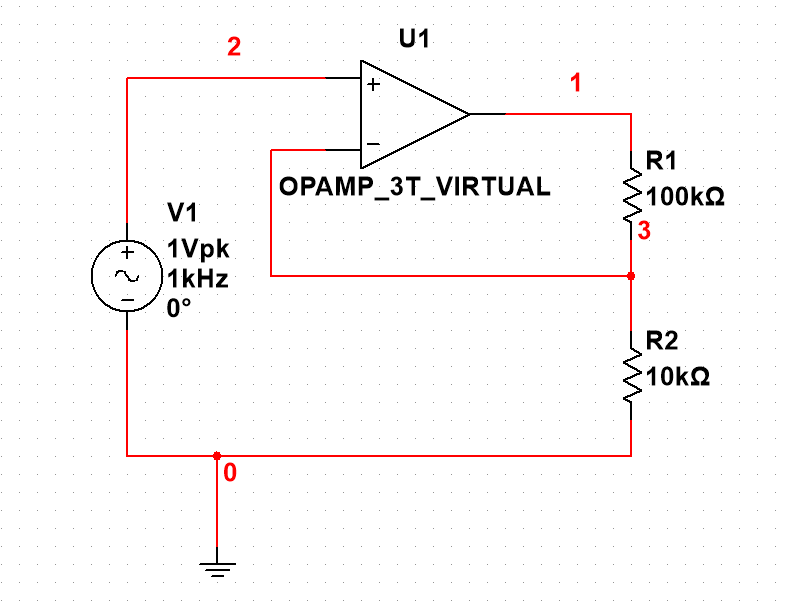
\includegraphics[width=0.5\linewidth]{neinv_zesilovac.png}
    \caption{Neinvertující zesilovač, zde $G = 11$}
    \label{fig:neinv_zesilovac}
\end{figure}

Na obrázcích \ref{fig:bode_neinv_2} a \ref{fig:bode_neinv_11} jsou frekvenční charakteristiky pro obě zadaná zesílení.
Pro $G = 2$ je $f_m \approx 500 \si{\kilo\hertz}$, pro $G = 11$ je $f_m \approx 90 \si{\kilo\hertz}$.
Pro simulaci byl použit tranzitní kmitočet $f_T = 1 \si{\mega\hertz}$, obě konfigurace
proto splňují rovnost $G \cdot f_m = f_T$, takzvaný \textit{gain-bandwidth product}.

\begin{figure}[h!]
    \centering
    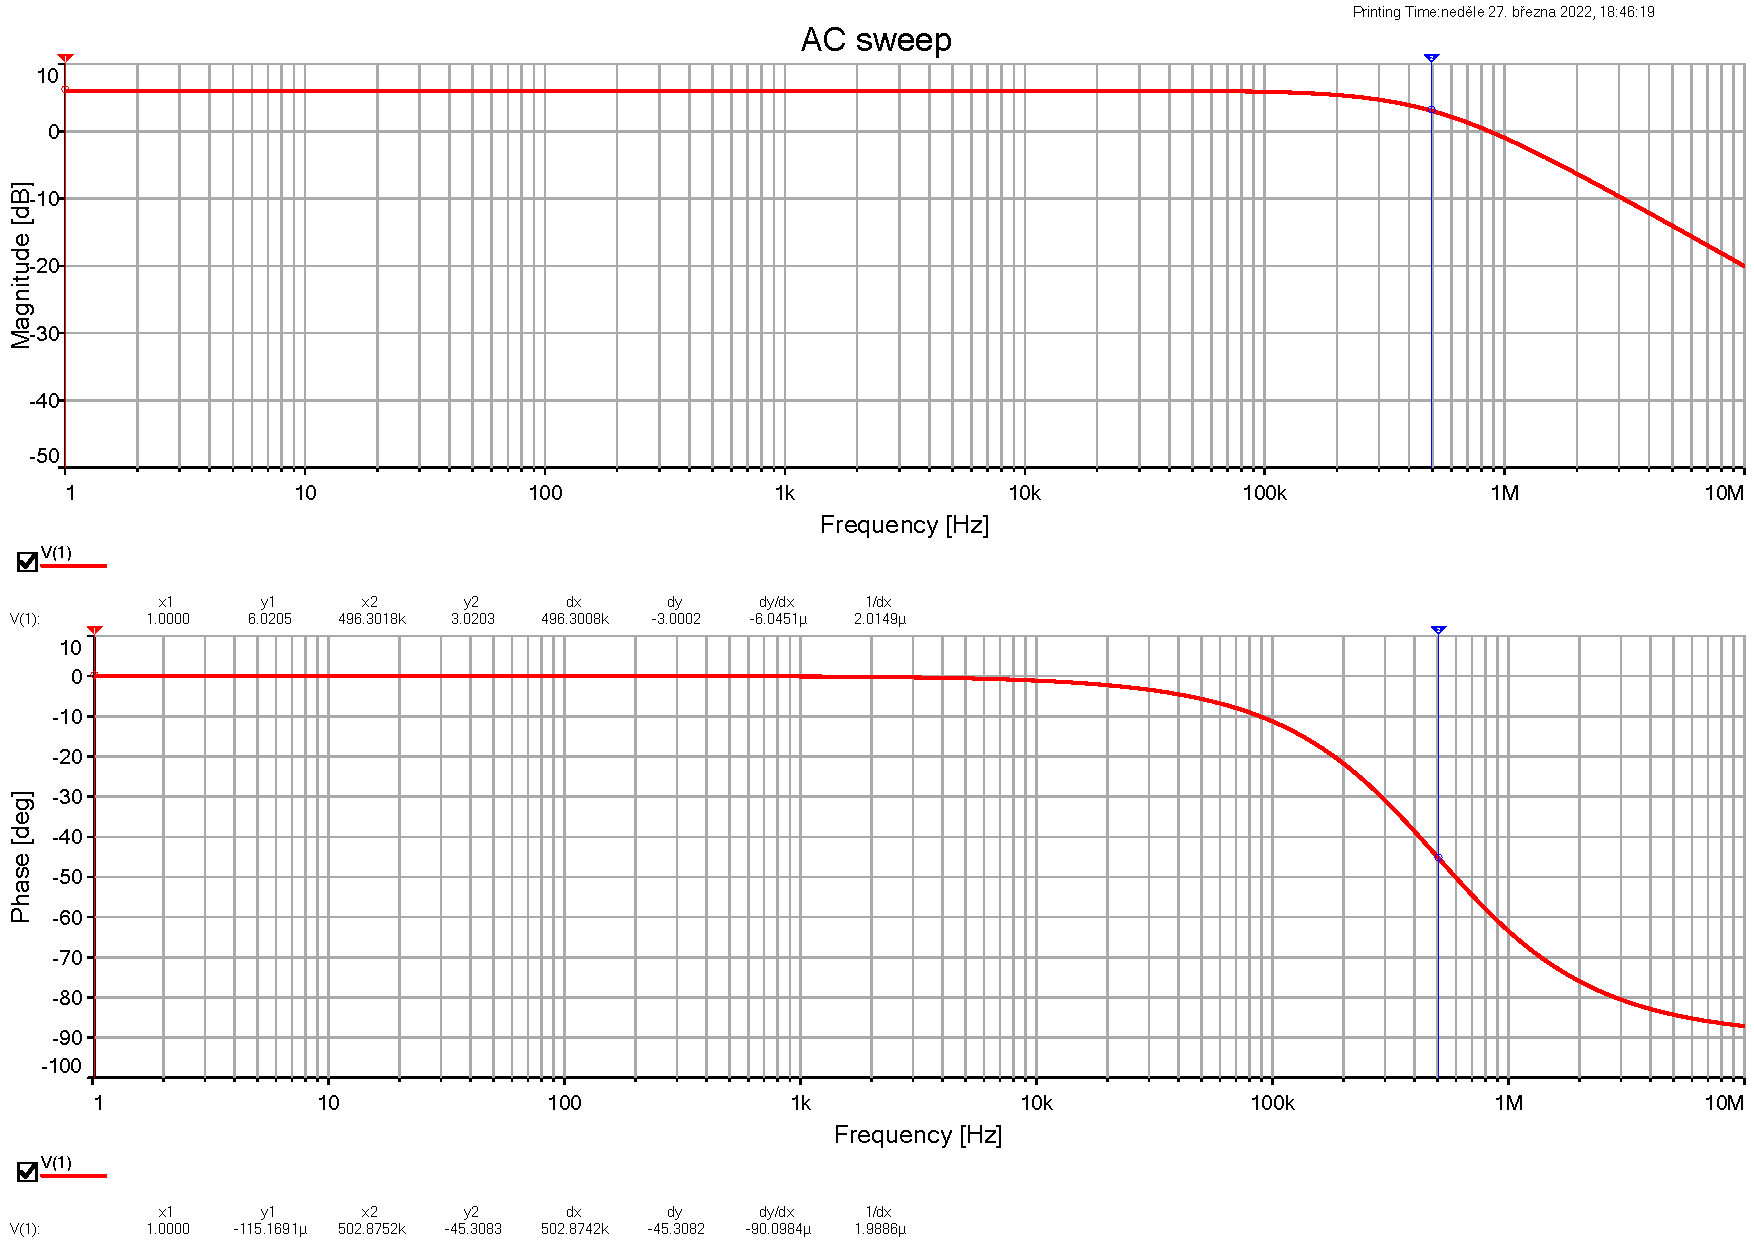
\includegraphics[width=0.92\linewidth]{bode_noninv_2.pdf}
    \caption{Frekvenční charakteristika neinvertujícího zesilovače pro $G=2$}
    \label{fig:bode_neinv_2}
\end{figure}

\begin{figure}[h!]
    \centering
    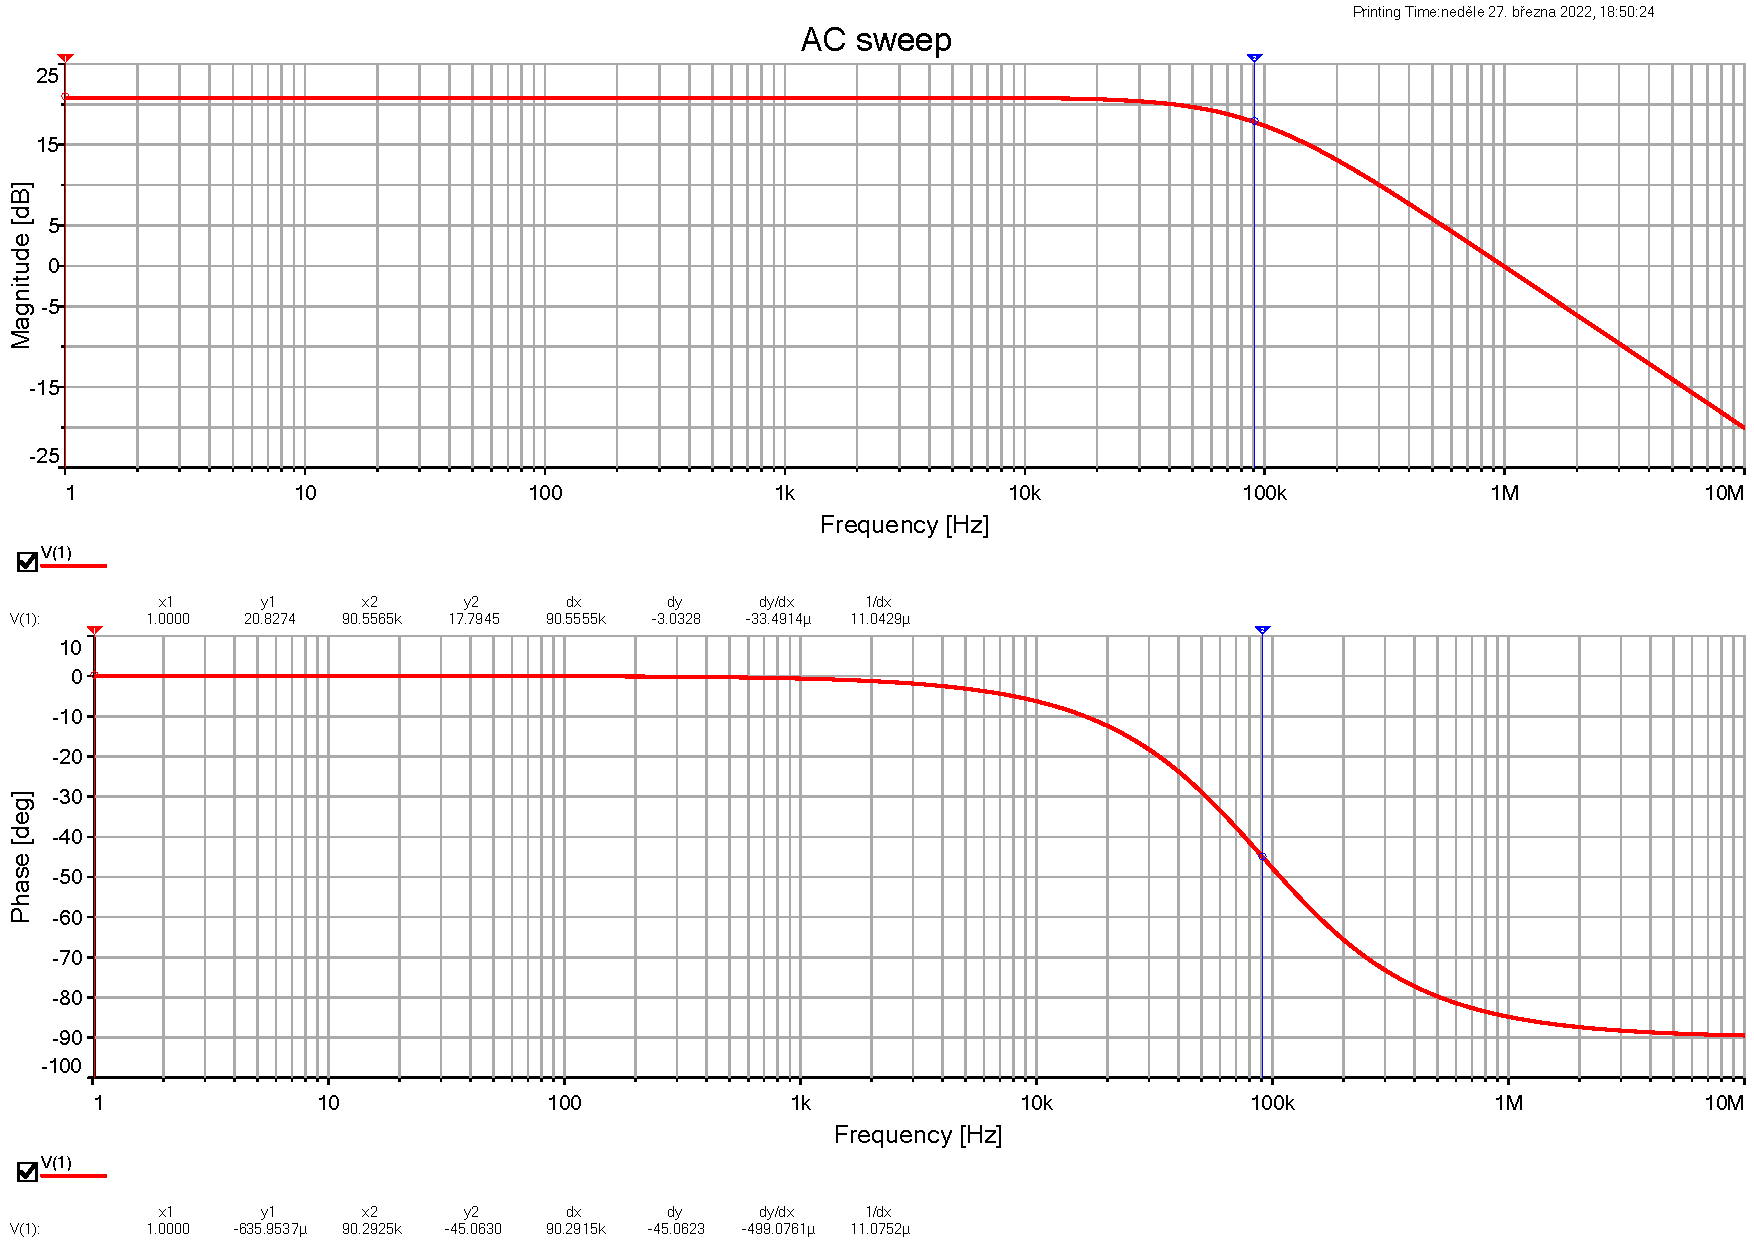
\includegraphics[width=0.92\linewidth]{bode_noninv_11.pdf}
    \caption{Frekvenční charakteristika neinvertujícího zesilovače pro $G=11$}
    \label{fig:bode_neinv_11}
\end{figure}

\newpage

Nahrazením harmonického buzení za obdélníkové \textit{clock voltage} je možné změřit dobu náběhu.
Na uvedených obrázkách přísluší zelený průběh vstupnímu obdélníkovému signálu, zatímco
červený průběh je napětí na výstupu zesilovače.
S použitím amplitudy vstupního signálu $U_1 = 909 \si{\milli\volt}$ a zesílením $G = 11$
je ustálené napětí rovno 10 \si{\volt}, pro což lze snadno dopočítat úrovně 10 a 90 \%.
Na obrázku \ref{fig:neinv_rise_time_11} je vidět doba náběhu mezi kurzory $T_n = 4,012 \si{\micro\second}$.

S použitím přibližného vztahu a změřené mezní frekvence $f_m$ pro $G = 11$ je očekávaná doba náběhu
\begin{equation}
    T_n = \frac{0,35}{90 \cdot 10^3} = 3,88 \si{\micro\second},
\end{equation}
což řádově odpovídá skutečné hodnotě změřené pomocí osciloskopu. Skutečná doba náběhu je trošku delší než teoretická,
jedním z důvodů je omezení derivace napětí na počátku konečnou rychlostí přeběhu (\textit{slew rate} $SR$).

Stejné měření lze provést pro zesílení $G = 2$, tedy $R_1 = R_2 = 10 \si{\kilo\ohm}$.
Na obrázku \ref{fig:neinv_rise_time_2} je zachycen průběh odezvy na skok, ze kterého lze
vyčíst doba náběhu $T_n \approx 690 \si{\nano\second}$, což odpovídá očekávané analyticky vypočtené hodnotě
\begin{equation}
    T_n \approx \frac{0,35}{500 \si{\kilo\hertz}} = 700 \si{\nano\second}.
\end{equation}

Velikost rychlosti přeběhu se nepodařilo spolehlivě změřit s pomocí mezního výkonového kmitočtu,
protože deformace harmonického průběhu nebyla nikdy příliš patrná.
Na časovém průběhu napětí na výstupu OZ nebyl nikdy patrný bod, kde přeběh přechází z lineárního na exponenciální.
Proto byl proveden jen hrubý odhad z počátku odezvy na jednotkový skok (s pomocí \textit{clock voltage}).
Na základě průběhu zobrazeného na obrázku \ref{fig:neinv_slew_rate} lze odhadnout
\begin{equation}
    SR = \frac{37,5 \si{\volt}}{8 \si{\micro\second}}  \approx 4,7 \si{\volt\per\micro\second}.
\end{equation}

\begin{figure}
    \centering
    \begin{subfigure}{0.45\textwidth}
        \centering
        
        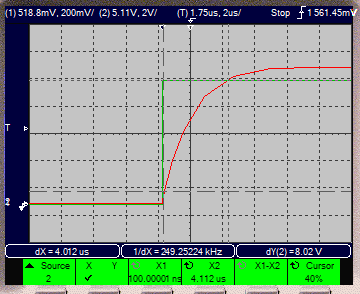
\includegraphics[width=0.8\linewidth]{neinv_rise_time_11.png}
        \caption{Pro $G=11$}
        \label{fig:neinv_rise_time_11}
    \end{subfigure}
    \begin{subfigure}{0.45\textwidth}
        \centering
        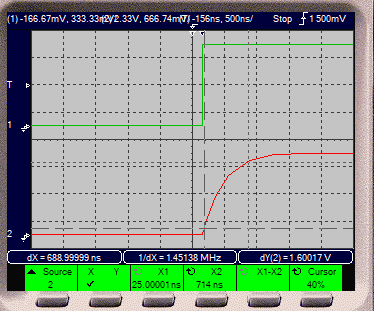
\includegraphics[width=0.8\linewidth]{neinv_rise_time_2.png}
        \caption{Pro $G=2$}
        \label{fig:neinv_rise_time_2}
    \end{subfigure}
    \caption{Měření doby náběhu $T_n$ neinvertujícího zapojení}
\end{figure}


\begin{figure}[h!]
    \centering
    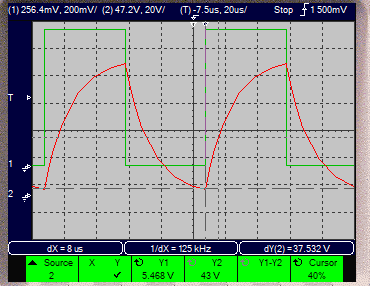
\includegraphics[width=0.50\linewidth]{neinv_slew_rate.png}
    \caption{Měření rychlosti přeběhu $SR$ zesilovače s $G=11$}
    \label{fig:neinv_slew_rate}
\end{figure}


\section{Invertující zesilovač}

Byl zapojen invertující zesilovač podle schématu \ref{fig:inv_zbytkove}.
Připojením vstupu na zem se projevily reálné vlastnosti operačního zesilovače:
\begin{enumerate}
    \item Napětí na invertující svorce je $u_- = - 1 \si{\milli\volt}$,
    což odpovídá očekávanému zbytkovému napětí použitého OZ.
    \item Vlivem rozdílu napětí teče přes rezistor $R_1$ proud $I_1 = 100 \si{\nano\ampere}$,
    z toho se $I_{BN} = 40 \si{\nano\ampere}$ ztrácí do invertující svorky OZ a zbylých $60 \si{\nano\ampere}$
    teče přes $R_2$ do výstupu OZ. Proto je výstupní napětí $u_{20} = -1,6 \si{\milli\volt}$.
\end{enumerate}

\begin{figure}[h!]
    \centering
    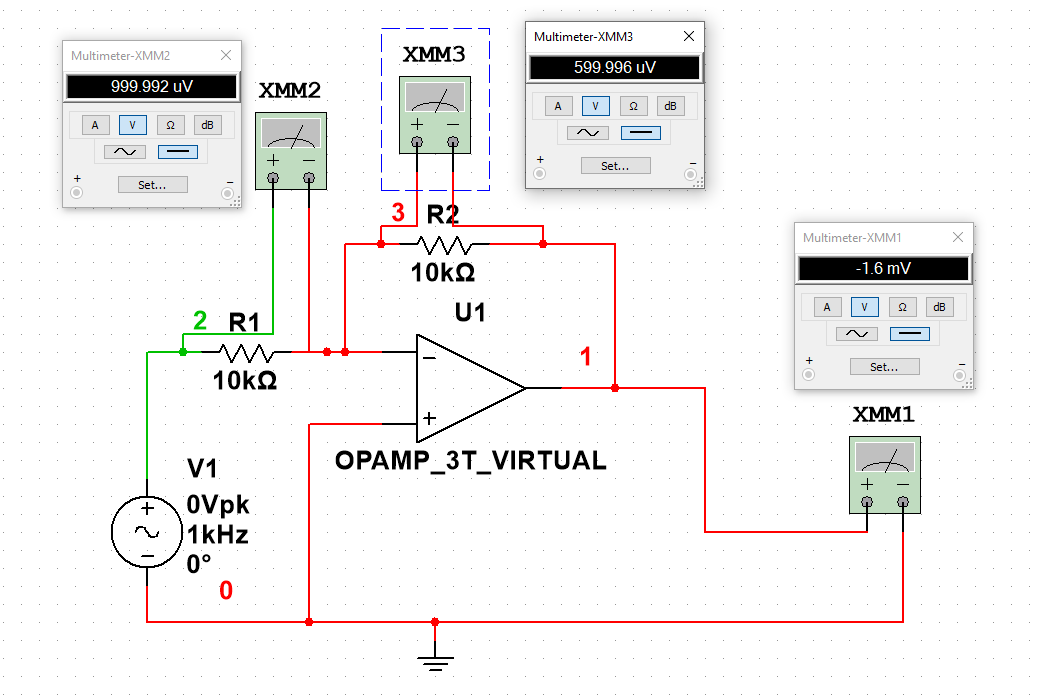
\includegraphics[width=0.7\linewidth]{inv_zbytkove.png}
    \caption{Zbytkové napětí invertujícího zesilovače}
    \label{fig:inv_zbytkove}
\end{figure}

Invertující zapojení operačního zesilovače má mezní kmitočet
\begin{equation}
    f_m = \frac{f_T}{1 + \vert G \vert},
\end{equation}
konfiguracím se zesílením $G_1 = -1$ a $G_2 = -10$ proto teoreticky přísluší mezní kmitočty
$f_{m_1} = 500 \si{\kilo\hertz}$ a $f_{m_2} = 90 \si{\kilo\hertz}$. Bodeho charakteristiky
vykreslené na obrázcích \ref{fig:bode_inv_1} a \ref{fig:bode_inv_10} tento teoretický 
předpoklad potvrzují simulací.

Reálná doba náběhu odpovídá, podobně jako u neinvertujícího zapojení, očekávané hodnotě
\begin{equation}
    T_n = \frac{0,35}{f_m}.
\end{equation}
Pro $G = -1$ je snímek časových průběhů z osciloskopu na obrázku \ref{fig:inv_rise_time_1},
ze kterého je patrno $T_n \approx 660 \si{\nano\second}$.

\begin{figure}[h!]
    \centering
    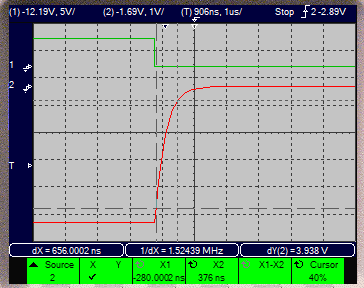
\includegraphics[width=0.35\linewidth]{inv_rise_time_1.png}
    \caption{Měření doby náběhu $T_n$ zesilovače s $G=-1$}
    \label{fig:inv_rise_time_1}
\end{figure}

\begin{figure}
    \centering
    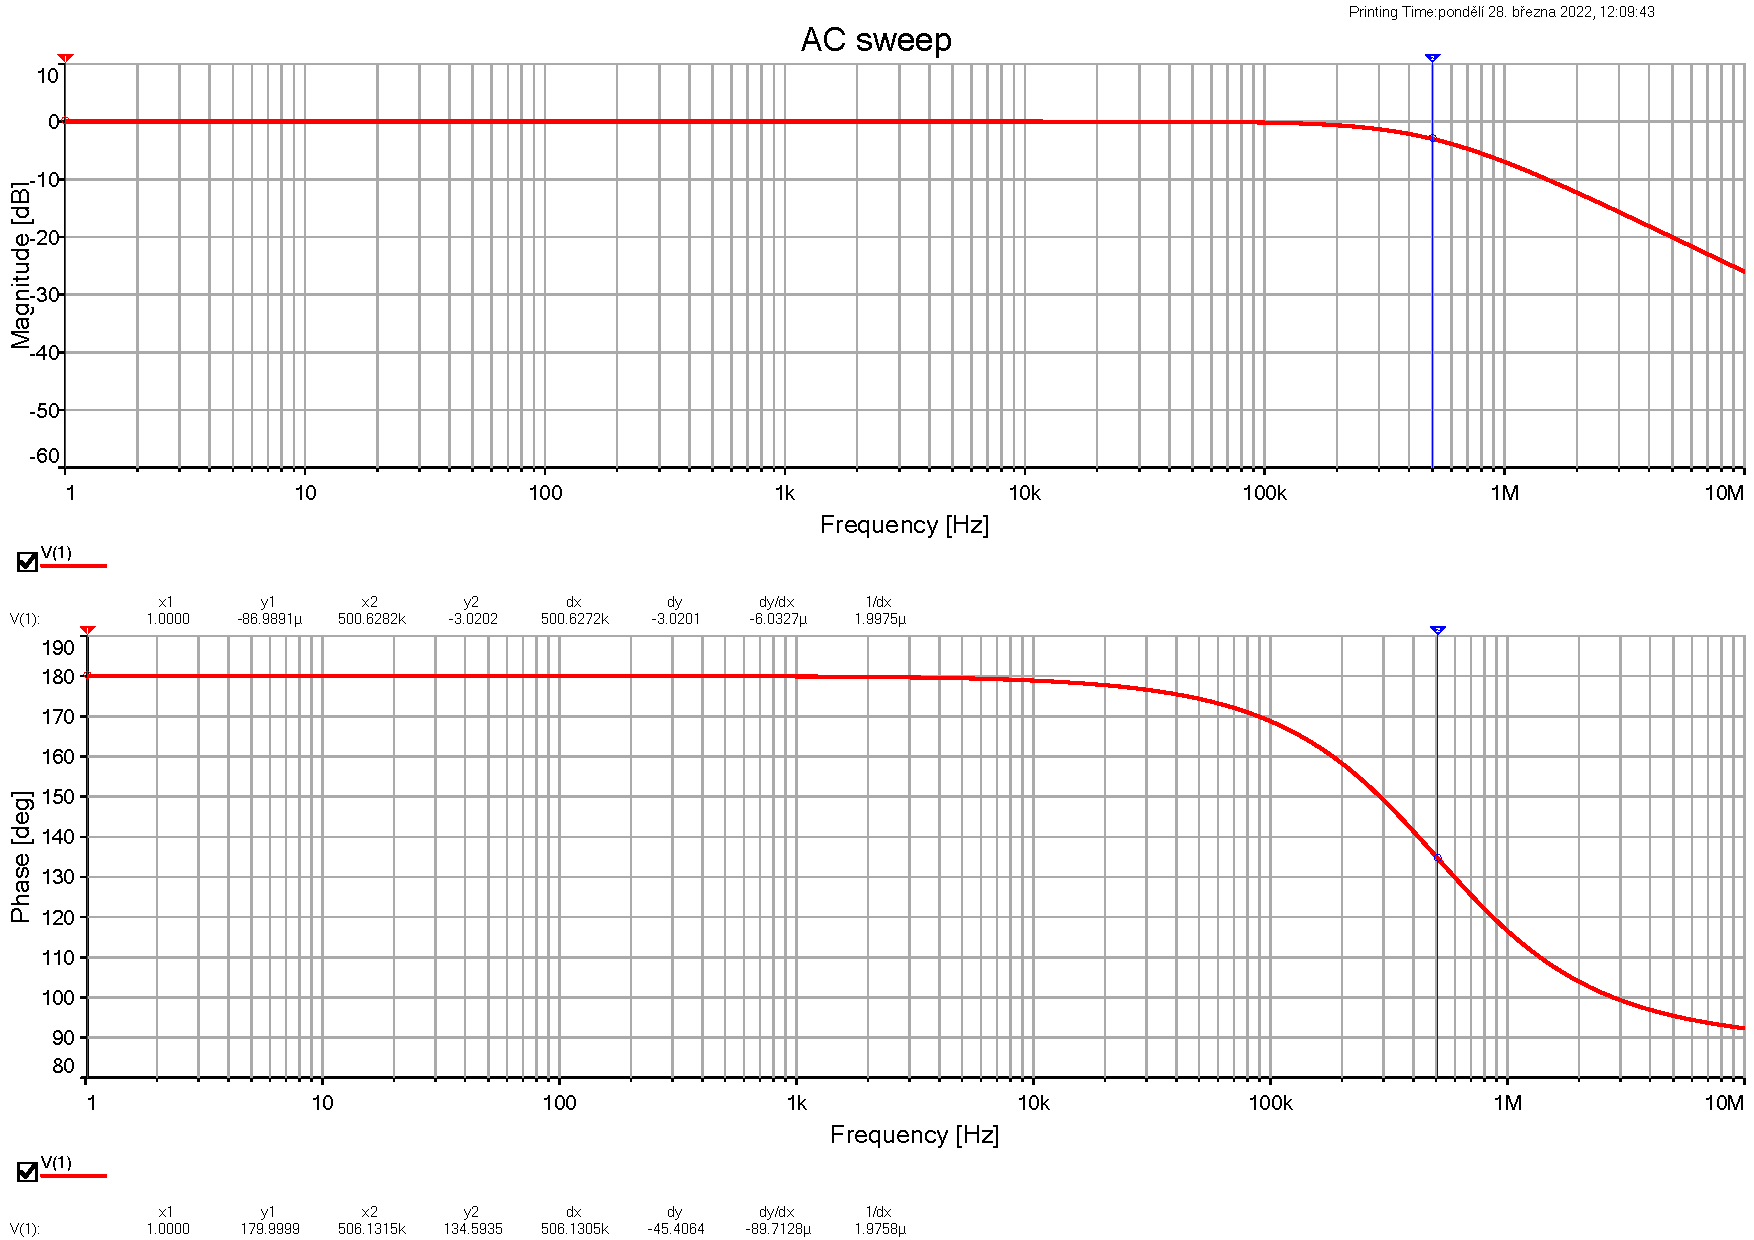
\includegraphics[width=0.92\linewidth]{bode_inv_1.pdf}
    \caption{Frekvenční charakteristika invertujícího zesilovače pro $G=-1$}
    \label{fig:bode_inv_1}
\end{figure}

\begin{figure}
    \centering
    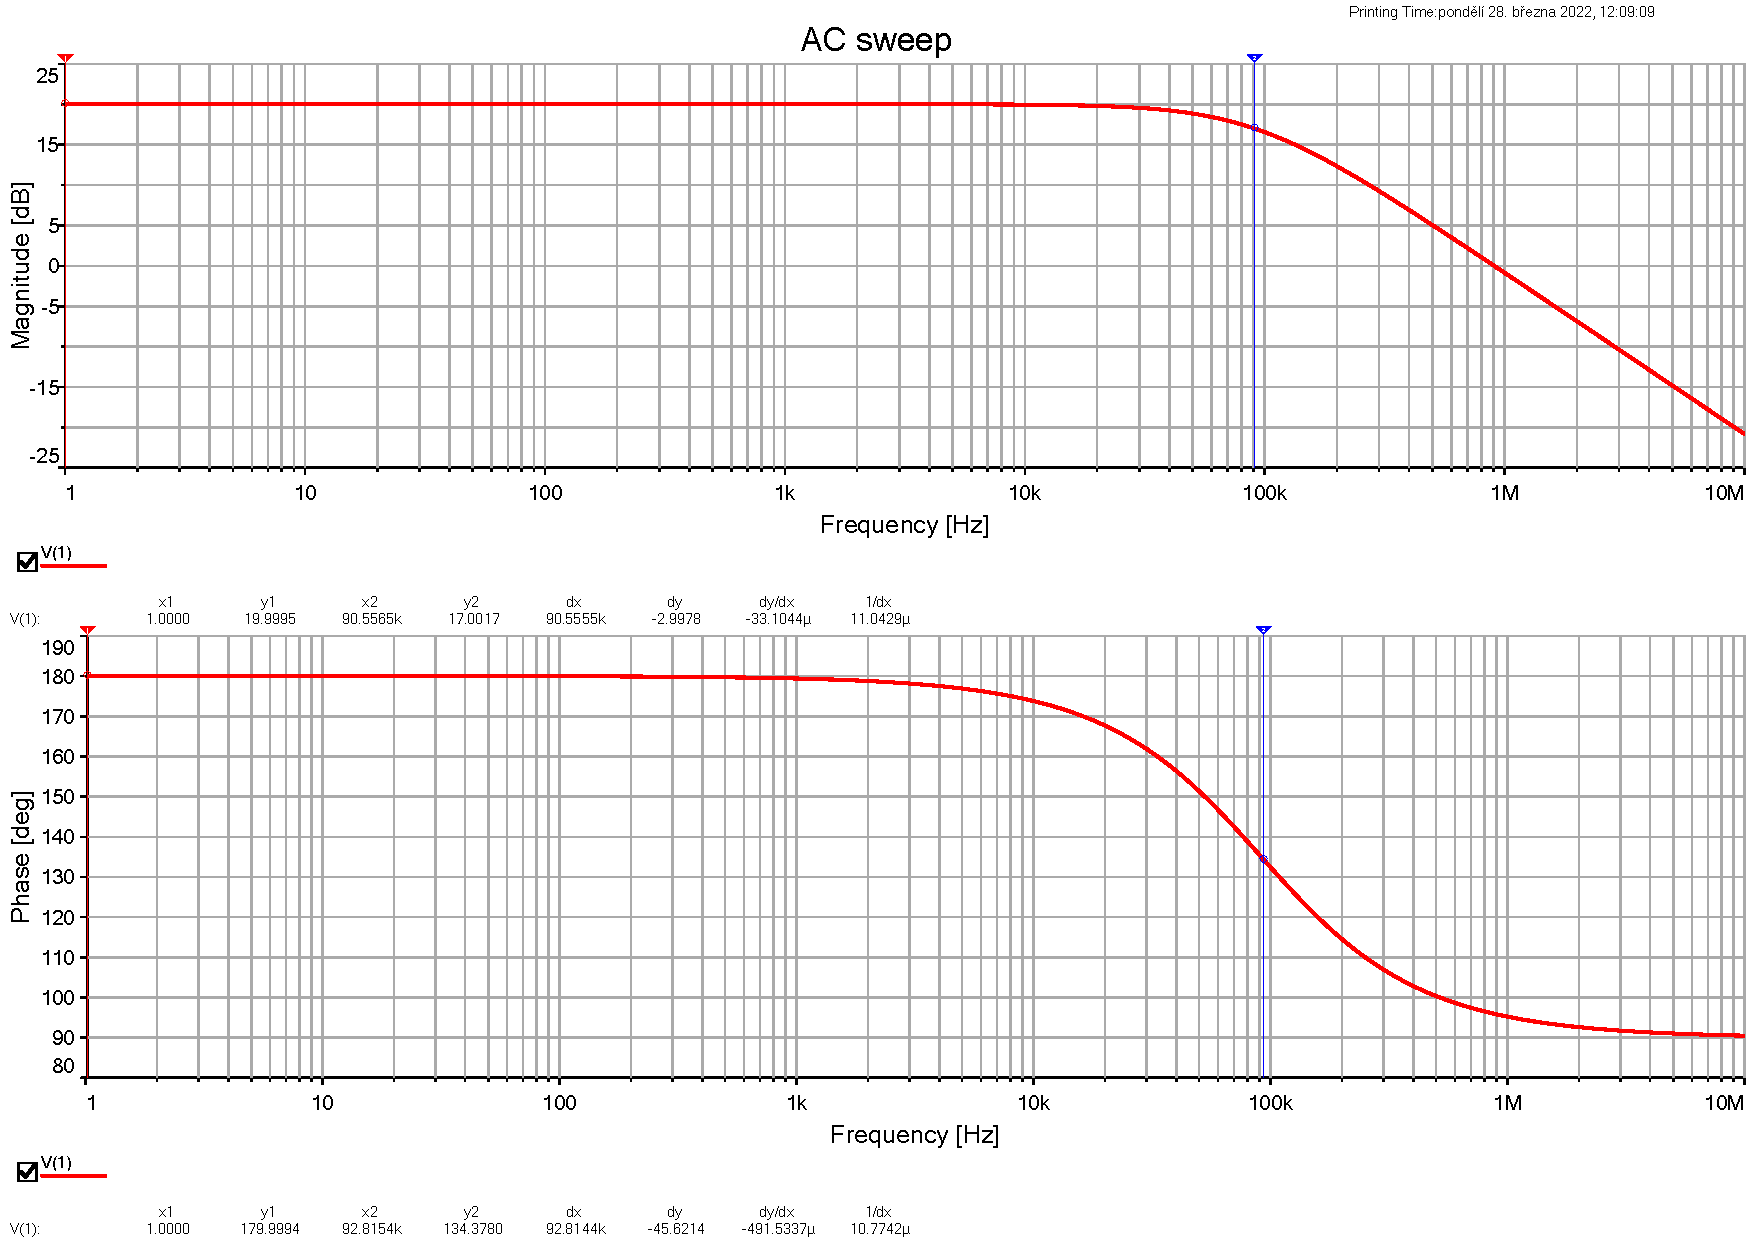
\includegraphics[width=0.92\linewidth]{bode_inv_10.pdf}
    \caption{Frekvenční charakteristika invertujícího zesilovače pro $G=-10$}
    \label{fig:bode_inv_10}
\end{figure}


\end{document}

